% Standalone source for the paper figure; build with figures/build.sh
\documentclass[border=1pt]{standalone}
% Shared preamble for the standalone figure sources.
\usepackage{times}
\usepackage{amsmath,amssymb}
\usepackage{xcolor}
\usepackage{textcomp}
\usepackage{tikz}
\usepackage{pgfplots}
\usetikzlibrary{arrows.meta,positioning,calc,fit,backgrounds}
\usepgfplotslibrary{fillbetween}
\pgfplotsset{compat=1.16}

% Colours are colour-blind safe (Okabe--Ito) and every figure also separates
% its classes by line style or fill, so the figures stay readable in greyscale.
\definecolor{cObs}{HTML}{0072B2}   % observed by the network
\definecolor{cHid}{HTML}{D55E00}   % hidden / unexplained
\definecolor{cHelp}{HTML}{009E73}  % safety helpers
\definecolor{cInk}{HTML}{333333}

\tikzset{
  box/.style={draw=cInk!70, rounded corners=1.5pt, fill=white, align=center,
              font=\scriptsize, inner sep=3pt, minimum height=0.8cm,
              line width=0.5pt},
  obs/.style={box, draw=cObs, fill=cObs!8},
  hid/.style={box, draw=cHid, fill=cHid!10},
  help/.style={box, draw=cHelp, fill=cHelp!10},
  flow/.style={-{Stealth[length=4pt]}, line width=0.6pt, draw=cInk!80},
  lbl/.style={font=\scriptsize, text=cInk!85, inner sep=1.5pt, align=center},
}
\pgfplotsset{
  every axis/.append style={font=\scriptsize, tick label style={font=\scriptsize},
                            label style={font=\scriptsize},
                            title style={font=\scriptsize\bfseries}, line width=0.5pt},
}

\begin{document}
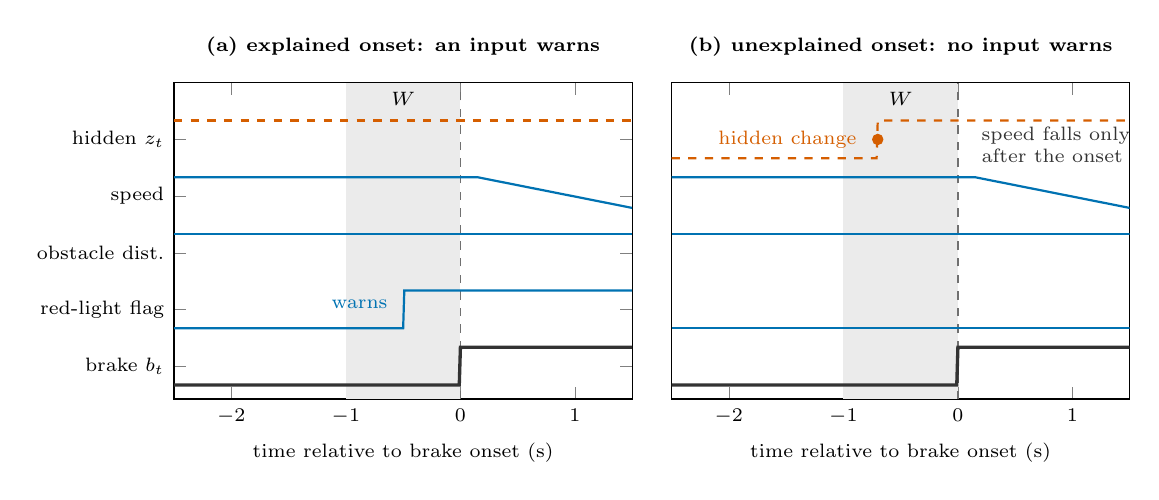
\begin{tikzpicture}
\begin{axis}[name=A, width=7.4cm, height=5.6cm, xmin=-2.5, xmax=1.5,
  ymin=-0.3, ymax=6.4, xlabel={time relative to brake onset (s)},
  ytick={0.4,1.6,2.8,4.0,5.2},
  yticklabels={brake $b_t$,red-light flag,obstacle dist.,speed,hidden $z_t$},
  xtick={-2,-1,0,1}, title={(a) explained onset: an input warns}]
  \fill[black!8] (axis cs:-1,-0.3) rectangle (axis cs:0,6.4);
  \node[font=\scriptsize] at (axis cs:-0.5,6.05) {$W$};
  \draw[dashed, cInk!70] (axis cs:0,-0.3) -- (axis cs:0,6.4);
  \addplot[cInk, very thick] coordinates {(-2.5,0)(-0.01,0)(0,0.8)(1.5,0.8)};
  \addplot[cObs, thick] coordinates {(-2.5,1.2)(-0.5,1.2)(-0.49,2.0)(1.5,2.0)};
  \addplot[cObs, thick] coordinates {(-2.5,3.2)(1.5,3.2)};
  \addplot[cObs, thick] coordinates {(-2.5,4.4)(0.15,4.4)(1.5,3.75)};
  \addplot[cHid, thick, dashed] coordinates {(-2.5,5.6)(1.5,5.6)};
  \node[font=\scriptsize, text=cObs, anchor=east] at (axis cs:-0.55,1.7) {warns};
\end{axis}
\begin{axis}[at={($(A.east)+(0.5cm,0)$)}, anchor=west, width=7.4cm, height=5.6cm,
  xmin=-2.5, xmax=1.5, ymin=-0.3, ymax=6.4,
  xlabel={time relative to brake onset (s)}, ytick=\empty, xtick={-2,-1,0,1},
  title={(b) unexplained onset: no input warns}]
  \fill[black!8] (axis cs:-1,-0.3) rectangle (axis cs:0,6.4);
  \node[font=\scriptsize] at (axis cs:-0.5,6.05) {$W$};
  \draw[dashed, cInk!70] (axis cs:0,-0.3) -- (axis cs:0,6.4);
  \addplot[cInk, very thick] coordinates {(-2.5,0)(-0.01,0)(0,0.8)(1.5,0.8)};
  \addplot[cObs, thick] coordinates {(-2.5,1.2)(1.5,1.2)};
  \addplot[cObs, thick] coordinates {(-2.5,3.2)(1.5,3.2)};
  \addplot[cObs, thick] coordinates {(-2.5,4.4)(0.15,4.4)(1.5,3.75)};
  \addplot[cHid, thick, dashed] coordinates {(-2.5,4.8)(-0.71,4.8)(-0.7,5.6)(1.5,5.6)};
  \addplot[only marks, mark=*, mark size=1.8pt, cHid] coordinates {(-0.7,5.2)};
  \node[font=\scriptsize, text=cHid, anchor=east] at (axis cs:-0.8,5.2) {hidden change};
  \node[font=\scriptsize, text=cInk, anchor=south west, align=left] at (axis cs:0.12,4.5)
    {speed falls only\\after the onset};
\end{axis}
\end{tikzpicture}
\end{document}
